\clearpage
\subsection{Nonlinear Optimization problem}
The objective is to minimize the following cost function:
\begin{align}
(B) : \hspace{2mm}
& \mbox{minimize} V (x) = - x_1 x_2 ; \ \  x \in \mathbb{R}^2 \nonumber \\
& \mbox{subject to : } \nonumber \\
& \hspace{2cm} h_1(x)= -x_1 - x_2^2 +1  \geq 0 \nonumber \\
& \hspace{2cm} h_2(x)= x_1 + x_2 \geq 0 \nonumber
\end{align}
This is a constrained nonlinear optimization problem of the form:
\begin{align}
    minimize \hspace{2mm} V(x) = f(x) \\
    subject\hspace{2mm} to\hspace{2mm} c(x) \geq 0 \\
    subject\hspace{2mm} to \hspace{2mm}h(x) = 0 \\
\end{align}
This can be solved using these algorithms: 
\begin{itemize}
    \item Penalty Function Algorithm
    \item Barrier Function Algorithm
    \item Augmented Lagragrian Algorithm
    \item Lagrange-Newton Algorithm
\end{itemize}
\subsubsection{Solutions to constrained nonlinear problem using our python programs and matlab benchmark \textit{fmincon} function: }
The algorithms converged to very close local minimal solutions for $x$ with a tolerance set to be $tol =1e-4$ and the same initial value of all column vector of $[5,5]^{T}$ as confirmed in the contour plot in figure 9.
The gradient loss of the penalty function converged to its minima in 2 iterations, while the newton Lagrangian took longest to converge using 3 iterations to converge. Unusually, our python solution converges faster than the matlab implementation that uses the interior point method. The solution from the newton Lagrangian and augmented newton method appears to be a long way off, as it lies on the intersections of the constraints of the contour plot. 
The contour graph of the function $V(x)$ and the minimum solutions of $x$ derived from the penalty algorithms showed that the lowest value of the objective function was at the intersection of the constraint ellipse and the contour graph of the objective function. 
\begin{table}[htbp]
\centering
\begin{center}
\begin{tabular}{|c|c|c|c|c|}
\hline
 & \textbf{Penalty} &\textbf{Aug Lag} &\textbf{Newton Lag} & \textbf{Matlab}\\
\hline
Iterations & 2 & 3 &2& 10 \\
\hline
$x$ & 
\begin{bmatrix}
0.6672 \\
0.5773 \\
\end{bmatrix}
&\begin{bmatrix}
 0.6178 \\
 -0.6182 \\
\end{bmatrix} &\begin{bmatrix}
 -1.6180 \\
 1.6180 \\
\end{bmatrix}
&\begin{bmatrix}
  0.6667 \\
 0.5774 \\
\end{bmatrix} \\ 
\hline 
\end{tabular}
\label{table:results}
\caption{Algorithm performance}
\end{center}
\end{table}

\begin{figure}[h!]
\centering
\begin{subfigure}[t]{0.4\textwidth}
\centering
    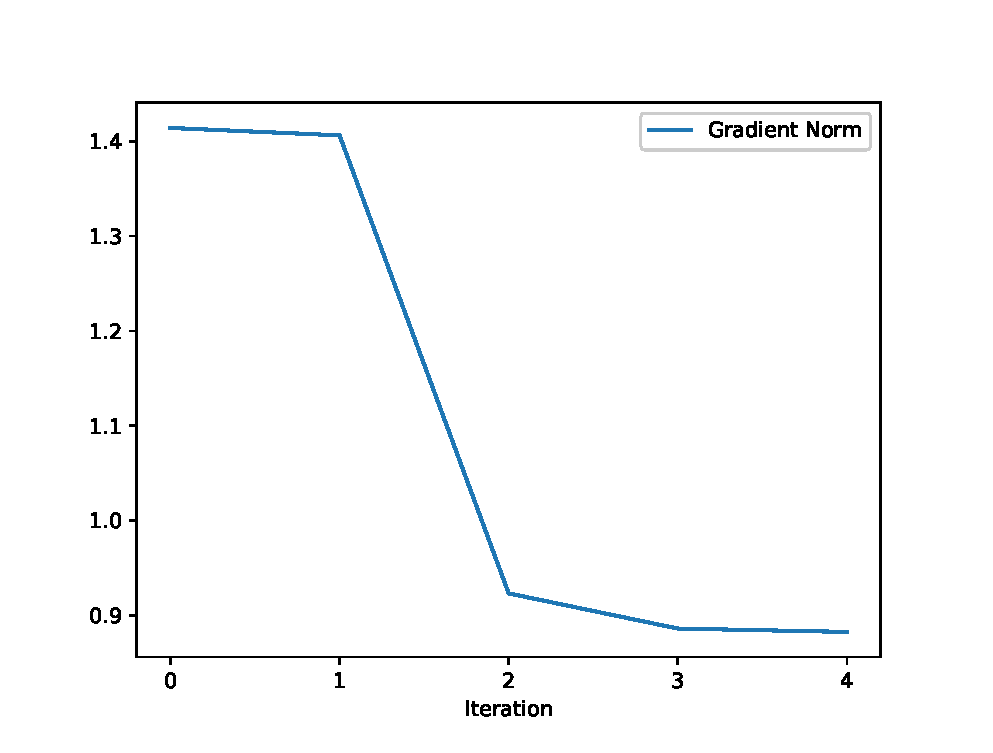
\includegraphics[width=\textwidth]{images/python/pe-pE.eps}
\caption{}
\label{fig:Class distribution}
\end{subfigure}
\hfill 
\begin{subfigure}[t]{0.4\textwidth}
\centering
    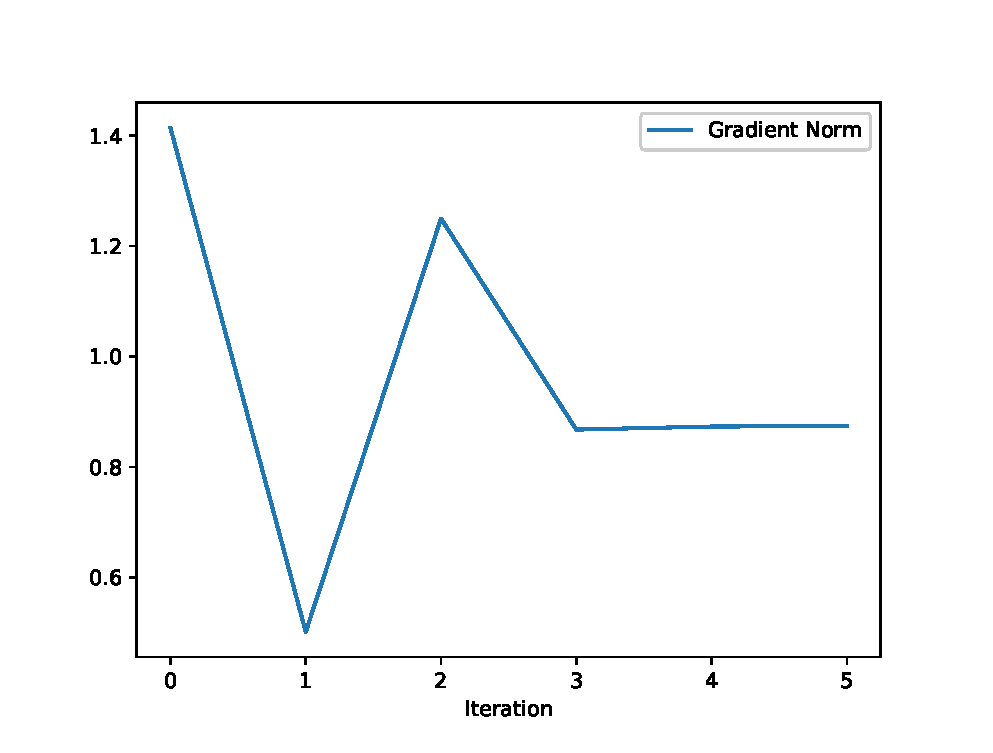
\includegraphics[width=\textwidth]{images/python/al-pE-ag.eps}
    \caption{}
    \label{fig:TSNE}
\end{subfigure}
\hfill
\begin{subfigure}[t]{0.4\textwidth}
\centering
    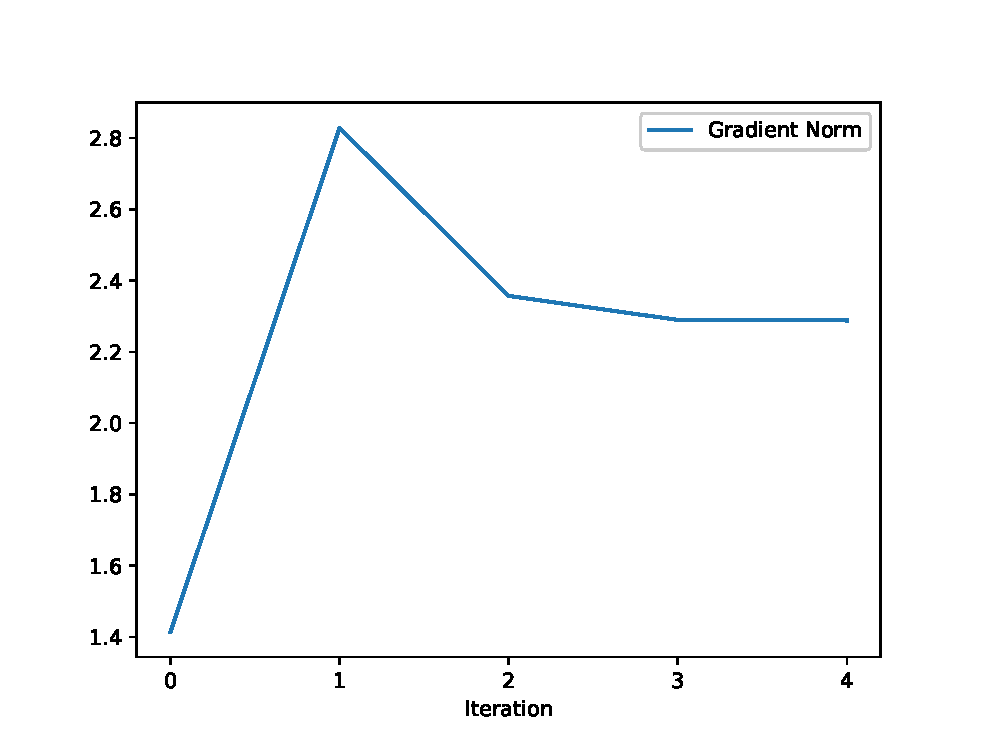
\includegraphics[width=\textwidth]{images/python/al-pE-ln.eps}
    \caption{}
    \label{fig:TSNE}
\end{subfigure}
\hfill
\begin{subfigure}[t]{0.4\textwidth}
\centering
    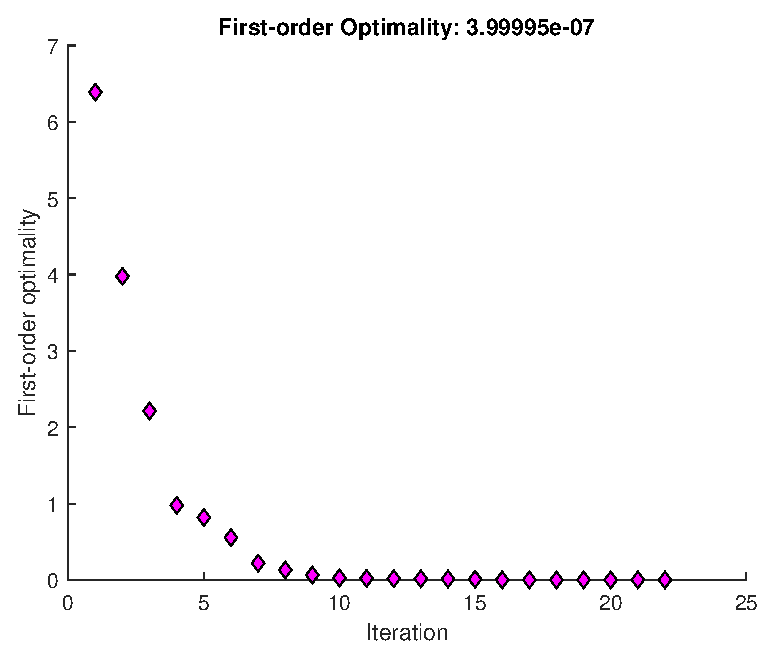
\includegraphics[width=\textwidth]{images/matlab/2b_loss.eps}
    \caption{}
    \label{fig:TSNE}
\end{subfigure}
\caption{(a): Penalty, (b): Augmented Lagrangian, (c): Newton Lagrangian, (d): Matlab: \textit{fmincon - interior - point}}
\end{figure}
\begin{figure}
    \centering
    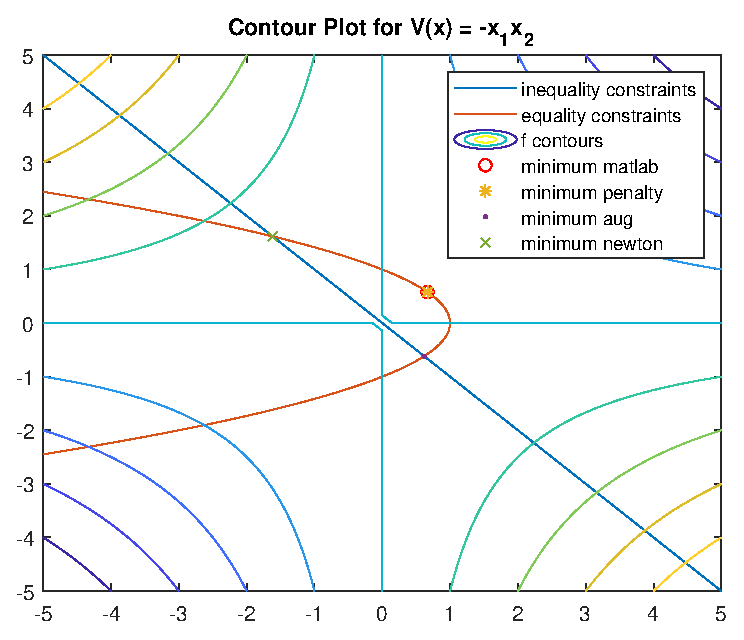
\includegraphics[width=0.4\textwidth]{images/matlab/matlab_2b.eps}
    \caption{Contour Plot for $V(x) =  V(x) = - x_1 x_2$ and its constraints}
\end{figure}